Our first real algorithm involves two parties, conventionally called \marginnote{
  \vspace{-80pt}
  \begin{center}
    \hspace{-10pt}
\includegraphics[width=0.95\linewidth]{img/letter}
  \end{center}  \vspace{-15pt}
  \emph{A letter from Alice. (Pun intended.)
  } \vspace{-10pt}
}
\textsc{Alice} and \textsc{Bob}, who wish to exchange a quantum state
at a distance. We assume this is a pure state of a qudit, $\psi = U
\triangleleft \pi^{(Z)}_0$ for some unitary $U$. 
We treat \texttt{U} and \texttt{d} as free parameters for now:
\begin{minted}
     [
frame=lines,
framesep=2mm,
baselinestretch=1.2,
bgcolor=AliceBlue,
fontsize=\footnotesize,
linenos
]{slurm}
    *> $alg = qudit(d)
    *> psi = U « char(Z, 0)
\end{minted}
To prepare the EPR state on a qudit, we follow the general recipe $\pi^{\text{(EPR)}}
= \text{CNOT}_d \triangleleft (\pi^{(X)}_0\otimes \pi^{(Z)}_0)$, outlined in
Exercise 3.2:
\begin{minted}
     [
frame=lines,
framesep=2mm,
baselinestretch=1.2,
bgcolor=AliceBlue,
fontsize=\footnotesize,
linenos
]{slurm}
    *> CNOT = sum(proj(Z,k) @ X**k for k in range(d))
    *> EPR = CNOT « char(X, 0) @ char(Z, 0)
\end{minted}
We suppose that Alice holds the state $\psi$, and shares the EPR state 
with Bob, so the total initial state is
\begin{minted}
     [
frame=lines,
framesep=2mm,
baselinestretch=1.2,
bgcolor=AliceBlue,
fontsize=\footnotesize,
linenos
]{slurm}
    *> init = psi @ EPR
\end{minted}

In order to transmit the state, we need to use a remarkable property
of the EPR state $\pi^{\text{(EPR)}}$ and its dual projector
$\Pi^{\text{(EPR)}}$ (see Exercise 4.2). For any operator $M \in
\mathcal{A}_d$,
\begin{align}
  \Pi^{\text{(EPR)}} \triangleright (M \otimes I) & =  \Pi^{\text{(EPR)}} \triangleright (I \otimes
                                                   M^\top) \label{eq:mirror1} \\  
  (M \otimes I) \triangleleft \pi^{\text{(EPR)}} & =   (I \otimes
                                                   M^\top) \triangleleft \pi^{\text{(EPR)}}. \label{eq:mirror2}
\end{align}
In words, we can apply $M$ to one end, or its transpose $M^\top$ to the other.
% It's a tricky to interpret the transpose in a purely
% algebraic way, so we can think of it in the GNS Hilbert space of
% $\pi^{(Z)}_0\otimes \pi^{(Z)}_0$ for
% convenience.
We won't define the transpose,\sidenote{If you are really curious,
  define $Z^\top = Z$, $X^\top = X^*$, and $(AB)^\top = B^\top A^\top$. % consider ``eigenoperators''
  % of the adjoint operation, $A^* = \omega A$, and define $A^\top =
  % \overline{\omega}A^*$.
} since all we need is that it is
``involutive'', $M^{\top\top} = M$.
% As you show in
% exercises, we can expand any $A \in \mathcal{A}_d$ in the so-called
% \emph{Weyl basis} of operators $W_{ab} = X^a Z^b$:
% \[
%   A = \sum_{a,b=0}^{d-1} c_{ab} W_{ab}.
% \]
The goal will be to use properties
(\ref{eq:mirror1})--(\ref{eq:mirror2}) on $U$, but that requires
an entangled \emph{measurement} on Alice's system. The simplest choice
is the \emph{Bell basis}
% to
% do that, Alice needs to entangle her state $\psi$ with her second
% state. The easiest way to do this is to measure in an entangled basis, with the canonical choice being
% the \emph{Bell basis} of Kraus operators:
\begin{equation}
  \label{eq:14}
\Pi^{\text{(EPR)}}_{ab} = (W_{ab}^* \otimes I) \triangleright \Pi^{\text{(EPR)}},
\end{equation}
where $W_{ab} = X^a Z^b$ is the \emph{Weyl operator basis} of $\mathcal{A}_d$
and
\[
  \Pi^{\text{(EPR)}}=\text{CNOT}_d^* \triangleright (\Pi^{(X)}_0 \otimes \Pi^{(Z)}_0)
\]
is the EPR projector dual to the EPR state $\pi^{(\text{EPR})}$.
In \texttt{yaw}, we implement the set $\Pi^{\text{(EPR)}}_{ab}$ as a list:
\begin{minted}
     [
frame=lines,
framesep=2mm,
baselinestretch=1.2,
bgcolor=AliceBlue,
fontsize=\footnotesize,
linenos
]{slurm}
    *> Pi = CNOT.d » proj(X, 0) @ proj(Z, 0)
    *> bell = [((X**a * Z**b @ I).d » Pi) @ I 
    ...               for a in range(d) for b in range(d)]
\end{minted}
Next, we measure in this basis, with post-measurement state
\texttt{post} and measurement outcome \texttt{index}:
  \begin{minted}
     [
frame=lines,
framesep=2mm,
baselinestretch=1.2,
bgcolor=AliceBlue,
fontsize=\footnotesize,
linenos
]{slurm}
    *> post, index = stMeasure(bell, init)()
\end{minted}
What does Alice learn from the value of \texttt{index}?
If Alice measures $a, b$, she applies the projector
$\Pi^{(\text{EPR})}_{ab}$ to her two qudits.
The end result is the entangled state $\pi^{(EPR)}_{ab}$ on her two
qudits and a disentangled state on Bob's.\sidenote{See the exercises
  for further discussion of this disentangling property of Bell
  measurements.}
% Our claim is Bob is not holding any old disentangled state, but a
% disguised version of Alice's $\psi$!
% To see why, consider Alice's projective
% measurement in the Bell basis.
When $U = I$ and $a, b = 0$, the resulting post-measurement state is
$\pi^{(\text{EPR})} \otimes \pi^{(Z)}_0$ as you can show in the exercises.
% $\pi^{(\text{EPR})}_{ab} \otimes (W_{ab}^*\triangleleft\pi^{(Z)}_0)$ for a general
% outcome.

What about nontrivial $U$?
%Here, (\ref{eq:mirror1}) comes to the rescue.
The only difference
between $U = I$ and general $U$ is a factor of $U \otimes I$ on
Alice's qudits, and by (\ref{eq:mirror1}),
\begin{align*}
\Pi^{(\text{EPR})}_{ab} \triangleright (U \otimes I) & =
                                                       \Pi^{(\text{EPR})}
                                                       \triangleright (W_{ab}^*U
                                                       \otimes I)\\
  & = \Pi^{(\text{EPR})} \triangleright \big(I \otimes (W_{ab}^*U)^\top\big).
\end{align*}
In effect, we have transferred $U$ (with correction) from Alice's
first qudit to the second.
% We can think of this operator now as acting on the entangled pair
% shared with Bob, and
Now we invoke (\ref{eq:mirror2}):
\begin{align}
  \label{eq:17}
\big(  (W_{ab}^*U)^\top \otimes I \big) \triangleleft \pi^{(\text{EPR})} & = \big(  I \otimes W_{ab}^*U \big) \triangleleft \pi^{(\text{EPR})},
\end{align}
using the fact $M^{\top\top} = M$.
% This suggests that Bob holds the operator $W_{ab}^* U$, applied to
% some state.
% This would be remarkable in itself, but even better, the state is
% precisely $W_{ab}^* U \triangleleft \pi^{(Z)}_0$, that is, Alice's
% state up to the correction
% $W_{ab}$.
% ``Mirroring'' suggests it should be the same one Alice used to
% prepare $\psi$, namely $\pi^{(Z)}_0$, and this turns out to be true!\sidenote{See the exercises to
% understand why.}
% As you can show in the exercises, when $U=I$,
Repeating the same disentangling measurement, we learn that the total
state is
\[
\pi^{(\text{EPR})}_{ab} \otimes (W_{ab}^*U\triangleleft\pi^{(Z)}_0).
\]
Thus, if Bob applies $W_{ab} = X^a Z^b$ to his qudit, he has $\psi$:
  \begin{minted}
     [
frame=lines,
framesep=2mm,
baselinestretch=1.2,
bgcolor=AliceBlue,
fontsize=\footnotesize,
linenos
]{slurm}
    *> a, b = index // d, index % d
    *> final = (I @ I @ (X**a * Z**b)) « post
\end{minted}
Here, \texttt{final} and \texttt{init} differ only in the location of
$\psi$.
\newpage

A cute way to check that this is indeed the state is to ``undo'' $U$ in Bob's
state \texttt{final}, i.e. apply $I \otimes I \otimes U^*$,
to nominally obtain $\pi^{(Z)}_0$ on Bob's system. Taking the expectation of $I
\otimes I \otimes Z$ then returns unity
just in case we genuinely have the state $\pi^{(Z)}_0$:\sidenote{A
  state with any variance in $Z$ must return an expectation with
  absolute value strictly less than $1$.}
  \begin{minted}
     [
frame=lines,
framesep=2mm,
baselinestretch=1.2,
bgcolor=AliceBlue,
fontsize=\footnotesize,
linenos
]{slurm}
    *> undo = (I @ I @ U.d) « final
    *> I @ I @ Z | undo
    1
\end{minted}
We collect the full protocol as a function of dimension and
unitary: \marginnote{
  \vspace{-45pt}
  \begin{center}
    \hspace{-10pt}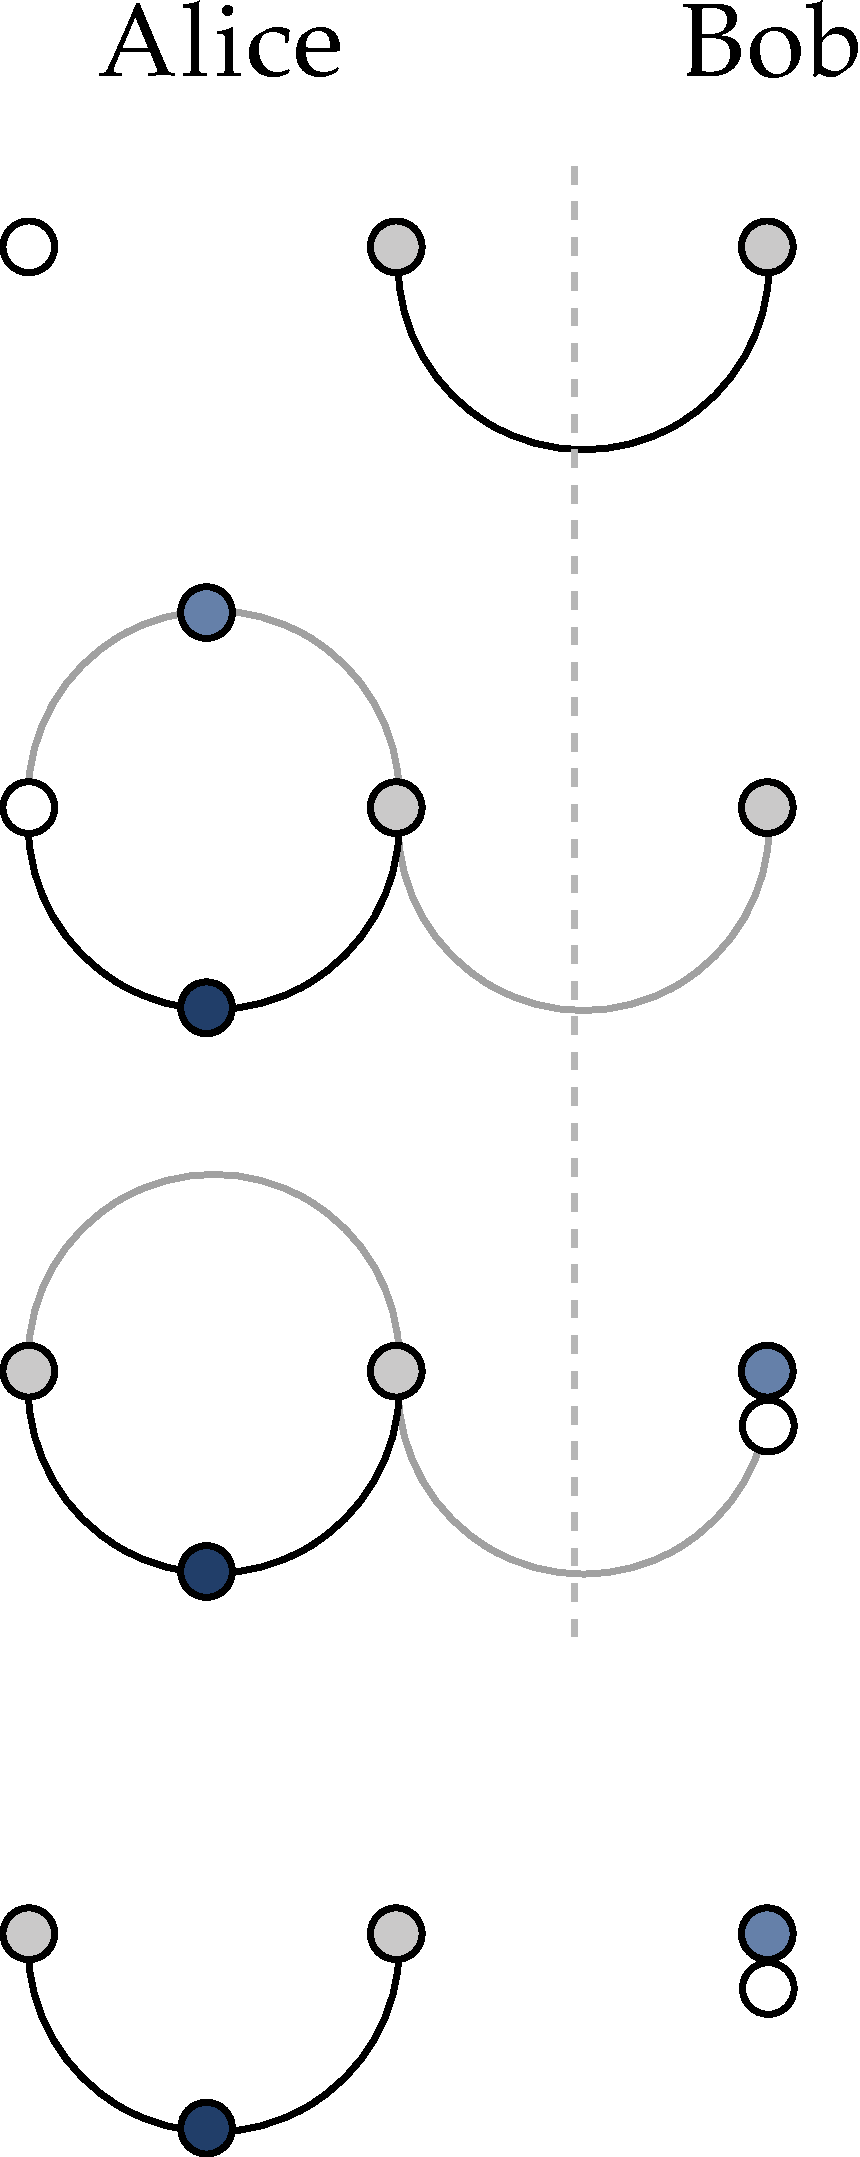
\includegraphics[width=0.6\linewidth]{img/teleport}
  \end{center}  \vspace{-0pt}
  \emph{1. A holds $U|0\rangle$; AB share an EPR
    pair. \\\hspace{-6pt}2. A measures in the Bell basis. \\\hspace{-6pt}3. The correction $W_{ab}^*$ and
    $U$ are mirrored. \\\hspace{-6pt}4. A has a Bell state and B has $W_{ab}^*U|0\rangle$.
  } \vspace{10pt}
}
  \begin{minted}
     [
frame=lines,
framesep=2mm,
baselinestretch=1.2,
bgcolor=AliceBlue,
fontsize=\footnotesize,
linenos
]{slurm}
    *> def teleport(d, U):
    ...   $alg = qudit(d)
    ...   CNOT = sum(proj(Z,k) @ X**k for k in range(d))
    ...   EPR = CNOT « char(X, 0) @ char(Z, 0)
    ...   init = (U « char(Z, 0)) @ EPR
    ...   Pi = CNOT.d » proj(X, 0) @ proj(Z, 0)
    ...   bell = [((X**a * Z**b @ I).d » Pi) @ I 
    ...              for a in range(d) for b in range(d)]
    ...   post, index = stMeasure(bell, init)()
    ...   return (I @ I @ (X**(index//d)*Z**(index%d))) « post
\end{minted}

Zooming out, why is this algorithm important? It shows that there is a
novel primitive in quantum computing: sending a quantum state. It
happens instantaneously, the moment Alice performs the Bell
measurement on her qudits, but is masked by the operator
$W_{ab}^*$ so that Alice must transmit the classical data $a$ and $b$ if Bob is to decode
the state he already has in his possession.\sidenote{You can explore the
causality-preserving aspects of this mechanism in the exercises.}
Teleportation and entanglement form the basis of an entirely new
discipline of \emph{quantum communication}, but we leave further
development of this subject
for another time.